%!TEX program = xelatex
\documentclass{article}
% \usepackage[UTF8,scheme=plain]{ctex}
\usepackage[a4paper,left=1.25in,right=1.25in,top=1in,bottom=1in]{geometry}

\usepackage{amsmath,amsthm,amsfonts,amssymb}
\usepackage{graphicx}
\usepackage{float}
\usepackage{subcaption}
\usepackage{booktabs,multirow,multicol}
\usepackage{indentfirst}
\usepackage{hyperref}
\usepackage{setspace}
\usepackage{listings}
\usepackage[ruled,noline]{algorithm2e}
\usepackage{bm}
\usepackage{xcolor}

\graphicspath{
    {./figure/}{./figures/}{./image/}{./images/}{./graphic/}{./graphics/}{./picture/}{./pictures/}
}

\lstdefinestyle{pythonstyle}{
    language=Python,
    basicstyle=\small\ttfamily,
    keywordstyle=\color{blue},
    commentstyle=\color{gray},
    stringstyle=\color{green},
    breaklines=true,
    showstringspaces=false,
    numbers=left,
    numberstyle=\footnotesize,
    frame=tb,
    columns=fullflexible,
    captionpos=b,
}

\title{Report Template}
\author{Author}
\date{\today}

\begin{document}
\maketitle

\section{Introduction}

This is where you describe the problems / goals of this report.

\section{Method}

Describe what you did. Did you have to innovate? Describe any
hurdles.

\subsection{Method 1}

Describe the numerical methods you employ.
If necessary, algorithms can be presented, for example, Algorithm~\ref{algorithm:1}.


\begin{algorithm}
    \caption{Euclid's algorithm}\label{algorithm:1}
    \KwData{Two nonnegative integers $a$ and $b$}
    \KwResult{Their greatest common divisor $d = \gcd(a, b)$}
    \While{$b \neq 0$}{
        $r \leftarrow a \bmod b$\;
        $a \leftarrow b$\;
        $b \leftarrow r$\;
    }
    $d \leftarrow a$\;
\end{algorithm}

\subsection{Method 2}

...

\section{Results}

Include and describe results obtained in this report.
You can make a table to show the accuracy results for your
method, e.g. Table~\ref{tab:demo0}.
You can also make a figure to show the results, e.g. Figure~\ref{fig:demo1} and Figure~\ref{fig:demo2}.


\begin{table}[ht]
    \centering
    \caption{Error and Order}\label{tab:demo0}
    \begin{tabular}{c|ccccc}
        \hline
                           & 10       & 20        & 40        & 80         & 160        \\
        \hline
        $L^{\infty}$~error & 0.283284 & 0.0758226 & 0.0192964 & 0.00484029 & 0.00121093 \\
        order              & -        & 1.90      & 1.97      & 2.00       & 2.00       \\
        \hline
    \end{tabular}
\end{table}

\begin{figure}[htbp]
    \centering
    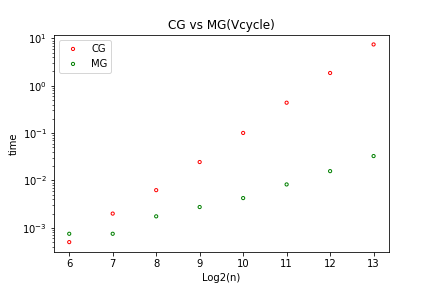
\includegraphics[width=.8\textwidth]{cg_mg.png}
    \caption{CG vs MG}\label{fig:demo1}
\end{figure}


\begin{figure}[htbp]
    \centering
    \begin{subfigure}[b]{0.47\textwidth}
        \centering
        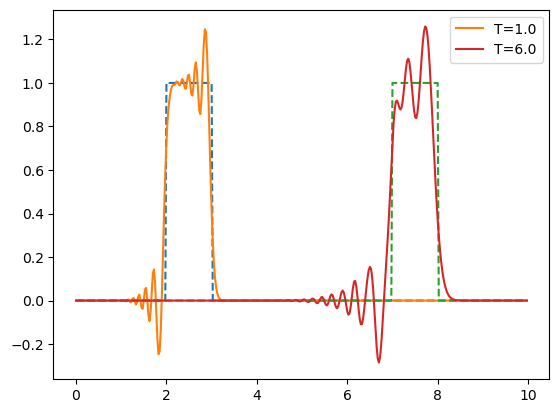
\includegraphics[width=\textwidth]{lw_r02.png}
        \caption{$R=0.2$}
        \label{fig:demo2-a}
    \end{subfigure}
    \begin{subfigure}[b]{0.47\textwidth}
        \centering
        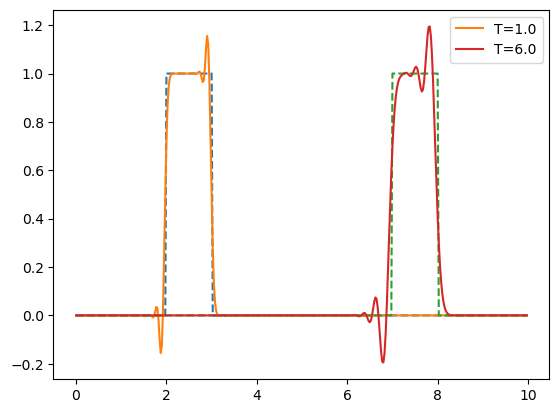
\includegraphics[width=\textwidth]{lw_r08.png}
        \caption{$R=0.8$}
        \label{fig:demo2-b}
    \end{subfigure}
    \caption{Demo}
    \label{fig:demo2}
\end{figure}

\section{Conclusion}

Summarize your findings and add your comments here.


\newpage

\appendix

\section{Computer Code}

Here we include the computer code.

\begin{lstlisting}[style=pythonstyle, caption=Demo, label=lst:python1]
def is_prime(num):
    """Check if a number is prime."""
    if num <= 1:
        return False
    if num <= 3:
        return True
    if num % 2 == 0 or num % 3 == 0:
        return False
    i = 5
    while i * i <= num:
        if num % i == 0 or num % (i + 2) == 0:
            return False
        i += 6
    return True

def generate_prime_numbers(n):
    """Generate the first n prime numbers."""
    count = 0
    current_number = 2
    while count < n:
        if is_prime(current_number):
            print(current_number)
            count += 1
        current_number += 1

# Test the function
generate_prime_numbers(20)
\end{lstlisting}



\end{document}
